% This is samplepaper.tex, a sample chapter demonstrating the
% LLNCS macro package for Springer Computer Science proceedings;
% Version 2.21 of 2022/01/12
%
\documentclass[runningheads]{llncs}
%
\usepackage[T1]{fontenc}
% T1 fonts will be used to generate the final print and online PDFs,
% so please use T1 fonts in your manuscript whenever possible.
% Other font encondings may result in incorrect characters.
%
\usepackage{graphicx}
% Used for displaying a sample figure. If possible, figure files should
% be included in EPS format.
%
% If you use the hyperref package, please uncomment the following two lines
% to display URLs in blue roman font according to Springer's eBook style:
% \usepackage{color}
% \renewcommand\UrlFont{\color{blue}\rmfamily}
% \urlstyle{rm}
%

% 箇条書きで bullet を使用するため
\usepackage{enumitem}
\usepackage{amsfonts}

% Table の設定で必要
\usepackage{booktabs}
\usepackage{makecell}   % provides \shortstack
\usepackage{tabularx}      % the X column type
\renewcommand\arraystretch{1.35}  % taller rows once globally


\usepackage[most]{tcolorbox}
\usepackage{float}

% Table(Change Rates of LLM Performance Metrics (Relative to Base Method)) で必要
\usepackage{caption}
\usepackage[margin=1in]{geometry}
\usepackage{multirow}


\usepackage{listings}
\newtcblisting{promptbox}[2][]{          % #1 extra keys, #2 title text
  colback=gray!5,
  colframe=black!75,
  sharp corners,
  boxrule=0.8pt,
  fontupper=\ttfamily\small,
  listing only,
  listing engine=listings,
  breakable,
  enhanced,                              % enables boxed title tricks
  title=#2,                              % header text
  boxed title style={                    % header appearance
     colback=gray!50,
     colframe=black!75,
     sharp corners,
     boxrule=0.8pt,
  },
  attach boxed title to top left={       % pin header to frame
     xshift=2mm, yshift=-2mm
  },
  #1                                     % allow overrides
}


\usepackage{array, tabularx, makecell}
\newcolumntype{L}{>{\raggedright\arraybackslash}X} % ← 左寄せ X 列


\usepackage[backend=biber,style=numeric,sorting=none]{biblatex}
\addbibresource{references.bib}

\begin{document}
%
\title{Prompt-Engineering Approaches \\to Reducing the Cost in LLM-Based Automated Test Case Generation}
%
\titlerunning{Prompt-Engineering Approaches to Reducing the Cost in LLM-Based Automated Test Case Generation}
%

\author{So Onishi\inst{1,2} \and
Keisuke Kitamura\inst{1,3} \and
Akihito Kohiga\inst{1,4} \and
Takahiro Koita\inst{1,5}}

%
\authorrunning{So Onishi et al.}
% First names are abbreviated in the running head.
% If there are more than two authors, 'et al.' is used.
%
\institute{Graduate School of Science and Engineering, \\Doshisha University, Kyotanabe, Kyoto, 619-0394, Japan \and
% \email{jt-koujm@mail.doshisha.ac.jp} \\
% \url{https://www.doshisha.ac.jp/en/} \and
\email{ctwk0154@mail4.doshisha.ac.jp} \and
\email{ctwn0119@mail4.doshisha.ac.jp} \and
\email{akohiga@mail.doshisha.ac.jp} \and
\email{tkoita@mail.doshisha.ac.jp}
}

%
\maketitle              % typeset the header of the contribution
%
\begin{abstract}
    % 114 words
Large language models (LLMs) can automate test case generation, but the prompts needed to reach coverage inflate tokens and API costs. We address this cost barrier by comparing two prompt-engineering strategies: (i) Docstring removal, (ii) LLMLingua-2 compression. The techniques were benchmarked on Python projects with three LLMs. LLMLingua-2 reduced API costs by 6.8\% without compromising the code coverage rate, which remained at 100\% code coverage. Docstrings removal cut cost for one model but increased it for the others, revealing model-specific dependencies on documentation quality. These results demonstrate that careful prompt-engineering can deliver predictable, low-risk savings, advancing the deployment of economical LLM-based test case generation.


    \keywords{Prompt-Engineering \and Token Reduction \and Natural Language Compression \and API Costs \and Code Documentation(Docstrings).}
\end{abstract}
%
%
%
\section{Introduction}
    Ensuring software reliability requires rigorous validation with a sufficient number of test cases, yet test case generation consumes about 15\% of developers’ working time and has long been a bottleneck, increasing maintenance overhead and causing schedule delays \cite{a_survey_on_unit_testing_practices_and_problems}. Traditional remedies—such as random testing and exploratory search—have been explored, but they rarely deliver stable, high code coverage.

The recent advent of large language models (LLMs) has changed the landscape: by supplying only source code or specifications, developers can automatically generate test cases that raise coverage while reducing manual effort, drawing rapid attention from both research and industry \cite{no_more_manual_tests?}. In fact, the 2024 Stack Overflow Developer Survey reports that 46.2\% of respondents are interested in introducing AI tools for test code, and more than 80\% believe such tools will be even more integrated into practice by 2025, underscoring the rising expectations for automated test case generation \cite{ai_in_the_development_workflow_interested,ai_tools_next_year}.

Nevertheless, today’s LLM-generated tests still pose quality challenges \cite{the_good_the_bad}: 

\begin{enumerate}[label=(\roman*)]
    \item Some fail to compile or crash at runtime
\vspace{0.2cm}
    \item Many are redundant yet still fall short on coverage
\vspace{0.2cm}
    \item The stochastic nature of LLMs leads to output variability and poor reproducibility
\end{enumerate}

Previous studies focus on that achieving high coverage requires providing the LLMs with large contextual information. Concrete proposals include method slicing, which decomposes complex functions into condition- or feature-level slices and generates test cases for each, and multi-step reasoning that feeds back coverage metrics to iteratively refine the tests; these approaches improve coverage and quality \cite{hits}.
% concreate: 具体的な

However, these techniques expand the amount of information and the number of tokens turn in the prompt. Then API costs rise nearly linearly with that count. Hence, deploying LLM-based test case generation in real projects demands strategies that controls cost increases caused by prompt bloat while preserving high coverage and quality.

To summarize, the key motivations and challenges addressed in this study are as follows:

\begin{itemize}[label={$\bullet$}]
    \item \textbf{Test case generation remains costly and time-consuming}: consuming 15\% of developers’ working time and contributing to delays and maintenance overhead.
    \vspace{0.2cm}
    
    \item \textbf{Existing methods to get high coverage}: such as method slicing and iterative feedback using coverage metrics—\textbf{require feeding large contextual information} to the LLMs, leading to prompt bloat.
    \vspace{0.2cm}
    
    \item \textbf{Prompt bloat increases tokens}: which in turn causes higher API costs for LLMs, posing a barrier to practical adoption.
\end{itemize}

The main contribution of this paper is to demonstrate that natural language compression and docstrings optimization can significantly reduce tokens and API costs while preserving 100\% code coverage. These results demonstrate that prompt-engineering can deliver predictable cost saving, advancing the deployment of economical LLM-based test case generation.


\section{Related Works}
    The use of LLMs for automating test case generation has garnered significant attention. A number of methods have been proposed with the goal of improving code coverage. One such approach is HITS (Hierarchical Test Generation with Slicing) by Wang et al., which introduces a method of semantically dividing the target method into multiple “slices,” generating individual prompts for each, and integrating the resulting test cases \cite{hits}. This technique has demonstrated superior coverage compared to existing methods such as ChatUniTest, SymPrompt, and EvoSuite. Notably, it achieved an average statement coverage of 55.09\% and branch coverage of 48.12\% on complex Java methods.

However, these improvements in coverage come with trade-offs. The increase in prompt granularity and repeated interactions with the LLMs for each slice significantly inflates the total token count, leading to a sharp rise in API usage costs. This introduces a new challenge: balancing performance gains against the growing computational and financial overhead.

Another area gaining attention is the role of contextual information—specifically, in-code documentation such as comments and docstrings as shown blue lines in Fig.\ref{fig:ex_docstrings}—in influencing the performance of LLMs. Macke et al. quantitatively evaluated how the presence and accuracy of documentation affect LLMs comprehension and generation capabilities \cite{testing_the_effect_of_code_documentation}. Their findings revealed that incorrect documentation can severely degrade performance. For instance, when random, misleading comments contradicting the code were provided, GPT-3.5’s accuracy dropped to 22.1\%, with a increase in runtime errors. These results underscore the importance of not simply maximizing prompt content, but ensuring the accuracy and relevance of included information especially in the context of test case generation.

To address the token inflation problem, recent studies have focused on prompt compression and information extraction as strategies to streamline inputs. A representative example is LLMLingua-2 by Microsoft Research, which distills GPT-4’s knowledge into a lightweight language model that compresses natural language prompts by 2 to 5 times while retaining key information and maintaining task performance. Moreover, response times were accelerated by up to 2.9×, yielding efficiency gains in both cost and interaction latency. Although prompt compression has shown effectiveness in tasks such as natural language processing and code completion, its application in the domain of automated test case generation remains largely unexplored.

\begin{figure}
    \centering
    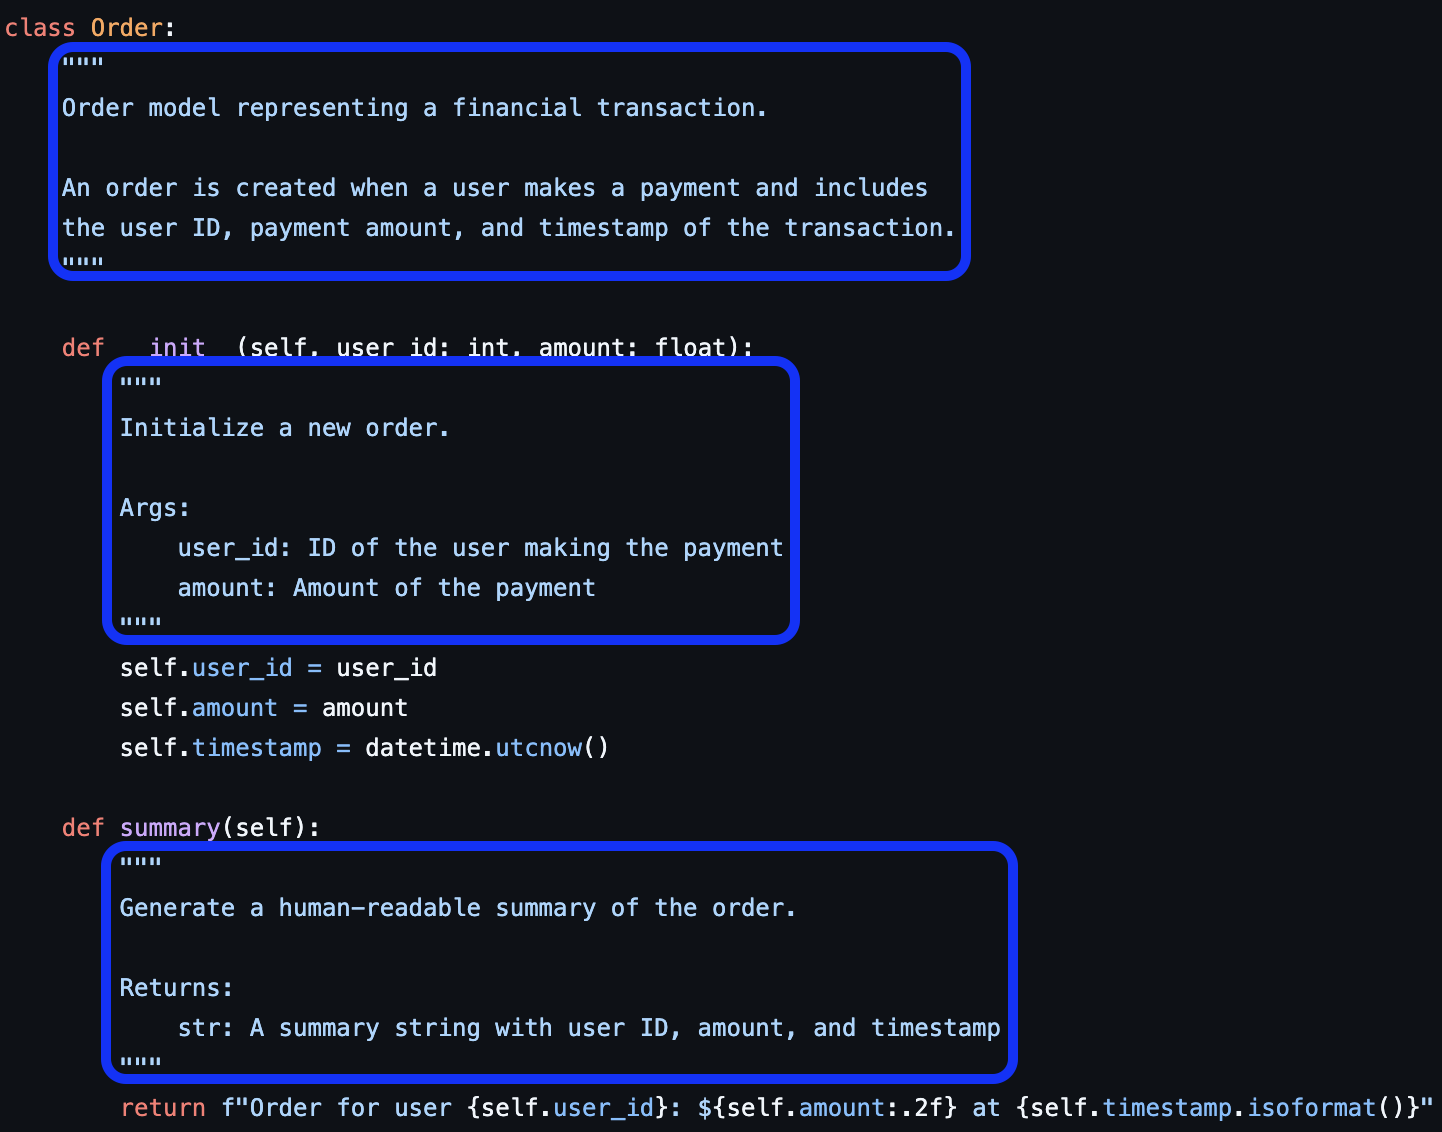
\includegraphics[width=0.8\linewidth]{imgs/png/docstrings.png}
    \caption{Example of Docstrings}
    \label{fig:ex_docstrings}
\end{figure}


\section{Objective}
    Most existing LLM-based test generation approaches still rely on incorporating extensive context—entire source files, function definitions, specifications, comments, and historical coverage data—into their prompts in pursuit of higher coverage. This inevitably exacerbates tokens and API cost.

In this research, we focus on the problem of prompt inflation in LLM-based test case generation. We propose a new method that leverages prompt-engineering to reduce input tokens while preserving generation quality, thereby reducing the overall number of tokens and API usage cost without sacrificing test effectiveness.


\section{Proposed Method}
    The core idea of the proposed method is to reduce input token counts in LLM-based test case generation while preserving generation quality. This study investigates three strategies:

\begin{enumerate}
    \item \textbf{Removal of in-code documentation of functions} (referred to as Docstrings in this study)
\vspace{0.2cm}
    \item \textbf{Natural language compression using LLMLingua-2}: applied to both prompts and Docstrings, to retain meaningful information while minimizing token count.
\end{enumerate}

\subsection{Role of LLMs in Test Case Generation}
LLMs are trained on extensive corpora of source code and natural language, enabling them to autonomously generate test code when provided with function specifications or intended behaviors. Given such prompts, LLMs can produce test cases that account for various edge cases and invalid inputs for function arguments, and even generate mocking logic for external API calls when necessary.

During this process, LLMs interpret the prompt—which includes instructions and code-related context—to infer the most appropriate and coverage-effective test scenarios. As a result, the quality and coverage of test cases generated by LLMs depend heavily on the content of the prompt. When the prompt includes sufficient context and clear guidance, LLMs can output test cases that closely resemble those written by human developers. Conversely, if the prompt lacks clarity or contains irrelevant or misleading information, the generated code may fail to compile or include redundant or ineffective test logic.

Therefore, prompt-engineering plays a critical role in maximizing the capabilities of LLMs and ensuring the generation of high-quality test cases.

\subsection{LLMs and AI Agent}
In this study, we adopt Claude 3.7 Sonnet, Gemini 2.5 Pro Preview, GPT-4.1 as LLMs. This decision is based on the two key considerations:

\begin{enumerate}
    \item All three models are offered by the top three vendors listed on Galileo's Agent Leaderboard on Hugging Face \cite{agent_leaderboard}. We selected the top-performing model from each vendor.
\vspace{0.2cm}
    \item To examine whether the results of the proposed prompt- engineering methods—such as Docstrings removal and natural language compression across different LLMs.
\end{enumerate}

The dataset used in this study, detailed later, includes functions with frequent cross-module calls, making it challenging for any LLMs to generate correct test code in a single prompt. Post-generation correction and retries are inevitable. As such, an automated framework capable of iterative test generation and error correction is essential.

To meet this need, we incorporate Cline, an open-source AI agent that facilitates autonomous iterative generation and correction. Cline offers the following key features:

\begin{itemize}[label={$\bullet$}]
    \item Plan Mode and Act Mode architecture, in which requirements and files are analyzed in Plan Mode and executed step-by-step in Act Mode based on a shared plan.
\vspace{0.2cm}
    \item Model-agnostic design, supporting multiple LLMs and enabling context windows exceeding 200k tokens. This allows for comprehensive analysis of entire codebases or multiple modules simultaneously.
\end{itemize}


\subsection{Prompt-Engineering}
Prompt-engineering refers to the practice of optimizing the input messages given to LLMs including system instructions, user queries, and contextual information to elicit desired and effective outputs \cite{llmlingua}. In the context of this study, the primary challenge of prompt-engineering is to selectively curate and concisely present the necessary information about the target code to LLMs, without including redundant or irrelevant details.

Traditionally, one might simply feed the entire source code and related documentation into the prompt and instruct LLMs to "generate test code for the given function." However, as discussed in the previous section, such prompts tend to become excessively verbose, leading to inefficiencies in both cost and performance. To address this, our study investigates the effect of reducing non-essential content in prompts—specifically, by removing Docstrings.

Docstrings are in-code natural language comments that describe what a function or class does and how it should be used. While potentially informative, they may not always contribute directly to generating effective test cases as I described in Section 2. Thus represent an opportunity for prompt reduction.

The base prompt used in this study is known as .clinerules, showed in Prompt 1. The .clinerules prompt is a type of custom instruction automatically inserted as a system prompt at the beginning of each Plan/Act step in the Cline framework. It defines coding standards, constraints, and recommended procedures to guide the LLM’s behavior.

\begin{promptbox}{Prompt 1: Base Prompt}
### Role

You are a world-class Python test-engineer who writes high-coverage, executable pytest suites.

### Scope

Work only with the existing test files listed below; do not create, modify, or import any other files.  
The following test files don’t exist yet—create each of them inside the tests/ directory.

- test_config.py
- test_data_generator.py
- test_main.py
- test_model_order.py
- test_model_user.py
- test_repository_order_repo.py
- test_repository_user_repo.py
- test_service_auth.py
- test_service_payment.py
- test_utils_math_utils.py
- test_utils_string_utils.py

### Goal

For this project (repository) **{{test_project_comments}}**, create tests that

- overall statement coverage must be ** 100% **,
- run without modification under `pytest`
  in tests folder.

### Task-breakdown

1. Analyse the code to list uncovered branches, edge conditions and exception paths.
2. Derive inputs that trigger each path.
3. Decide the expected output or raised exception.
4. Write a concise `pytest` function for every new case.
5. Re-scan to confirm no path remains untested.

### Constraints

- **Output code only** - no narrative, no comments, no docstrings.
- Do **not** add third-party dependencies.

### Generation checklist

- includes at least one exception/edge-case test
- hits every line shown as uncovered above
- all asserts use concrete literals
\end{promptbox}


In addition, all prompts are formatted using Markdown. Previous research has shown that presenting prompts in Markdown can improve LLMs response accuracy compared to plain-text formatting \cite{he2024doespromptformattingimpact}.

\subsection{Natural Language Compression}

To reduce prompt length, this study employs LLMLingua-2, a model designed for natural language compression \cite{pan2024llmlingua2datadistillationefficient}. LLMLingua-2 uses a token classifier to iteratively remove low-importance words, allowing it to achieve high compression rates while preserving semantic content. Previous research has shown that at a compression rate of 0.9 corresponding to a 5–10\% reduction in total tokens the performance drop is less than one percentage point. Based on this evidence, we adopt the same compression rate (0.9) in this study.

\subsubsection{Base Model}
The encoder used for LLMLingua-2 is mbert-base. Given that Docstrings typically consist of a few lines per code and follow standardized formats describing the purpose, parameters, and return values of functions, their lexical and syntactic variation is limited. As such, complex language phenomena requiring large-scale models are not expected to be present, making mbert-base a suitable and lightweight choice for this compression task.

In addition, because Docstrings are short by nature, we did not specify any mandatory tokens to preserve in LLMLingua-2. Specifically, the Tokens\_to\_Preserve parameter was set to an empty set (Ø), and the option to force preservation of tokens containing numeric values was disabled.

\subsubsection{Parameter Settings}
The LLMLingua-2 compression was applied using the following parameters:

\begin{itemize}[label={$\bullet$}]
    \item Base Model: mbert-base
\vspace{0.2cm}
    \item Tokens to Preserve: Ø
\vspace{0.2cm}
    \item Compression Rate: 0.9
\end{itemize}

Prompt 2 shows the result of compressing the original base prompt in Prompt 1.

\begin{promptbox}{Prompt 2: Compressed Prompt}
# # # Role You world - class Python test - engineer writes high - coverage, executable pytest suites. # # # Scope Work only with existing test files below ; do not create, modify, or import other files. following test files don t exist yet create each inside tests / directory. - test _ config. py - test _ data _ generator. py - test _ main. py - test _ model _ order. - test _ model _ user. - test _ repository _ order _ repo. py - test _ repository _ user _ repo. py - test _ service _ auth. py - test _ service _ payment. py - test _ utils _ math _ utils. py - test _ utils _ string _ utils. py # # # Goal For project ( repository ) * * { { test _ project _ comments } } * create tests overall statement coverage must be * * 100 % * *, - run without modification under pytest in tests folder. # # # Task - breakdown 1. Analyse code to list uncovered branches, edge conditions exception paths 2. Derive inputs trigger each path 3 Decide expected output or raised exception 4 Write concise pytest function for every new case. 5 Re - scan to confirm no path remains untested. # # # Constraints - Output code only * * no narrative, no comments, no docstrings. not * add third - party dependencies. # # # Generation checklist - includes at least one exception / edge - case test - hits every line shown as uncovered above - all asserts use concrete literals
\end{promptbox}


Table \ref{tab:token_reduction_llmlingua2} presents the number of tokens after applying LLMLingua-2 compression, along with the reduction rate compared to the base prompt. With the compression rate set to 0.9, the observed token reduction was approximately 11.2\%. Token counts were obtained using the official endpoint provided by Anthropic, the developer of Claude \footnote{\url{https://docs.anthropic.com/en/api/messages-count-tokens}}.

\begin{table}[h!]
  \centering
  \caption{Token Reduction by LLMLingua-2}
  \label{tab:token_reduction_llmlingua2}
  \begin{tabular}{|l|c|c|}
    \hline
    \textbf{Condition} & \textbf{Token Counts} & \textbf{Reduction Rate} \\
    \hline
    Prompt 1: Before Compression & 392 & -- \\
    Prompt 2: After Compression  & 348 & -11.2\% \\
    \hline
  \end{tabular}
\end{table}


\section{Experiment}
    This section describes the dataset, evaluation metrics, and experimental procedure used in this study.

\subsection{Dataset}

In this study, we used three types of Python project configurations as the dataset:

\begin{enumerate}
    \item Prompt + Docstrings \footnote{\url{https://github.com/soso0024/pj-aidev-dataset_prompt_docstrings}}
\vspace{0.2cm}
    \item Prompt Only \footnote{\url{https://github.com/soso0024/pj-aidev-dataset_prompt_only}}
\vspace{0.2cm}
    \item Compressed Prompt + Comprssed Docstrings (by LLMLingua-2) \footnote{\url{https://github.com/soso0024/pj-aidev-dataset_llmlingua-2}}
\end{enumerate}

Each configuration maintains identical function and class structures as well as dependency relationships. Only one factor changes are that whether the prompt and its docstrings are included and compressed. This setup allows for controlled evaluation of how natural language documentation—and its compression—affects the performance of LLM-based test case generation. 

The dataset emulates a complete financial-transaction workflow—user signup/login, balance tracking, payment processing, and order history—all on in-memory storage. The dataset offers the following key features:

\begin{itemize}[label={$\bullet$}]
    \item \textbf{Project Structure}:\\Each project is composed of the following directories: config/, data/, model/, repository/, service/, and utils/. Fig.\ref{fig:repository_visualization} shows a project visualization of the repository used in this study.
\vspace{0.2cm}
    \item \textbf{Code Formatting}:\\All repositories were formatted using Black to ensure consistent code style \footnote{\url{https://github.com/psf/black}}. Deviations from the formatting standard are detected via GitHub Actions using black\_formatter.yml. This enforcement ensures that differences in code style do not influence the experimental results.
\end{itemize}

\begin{figure}[htbp]
    \centering
    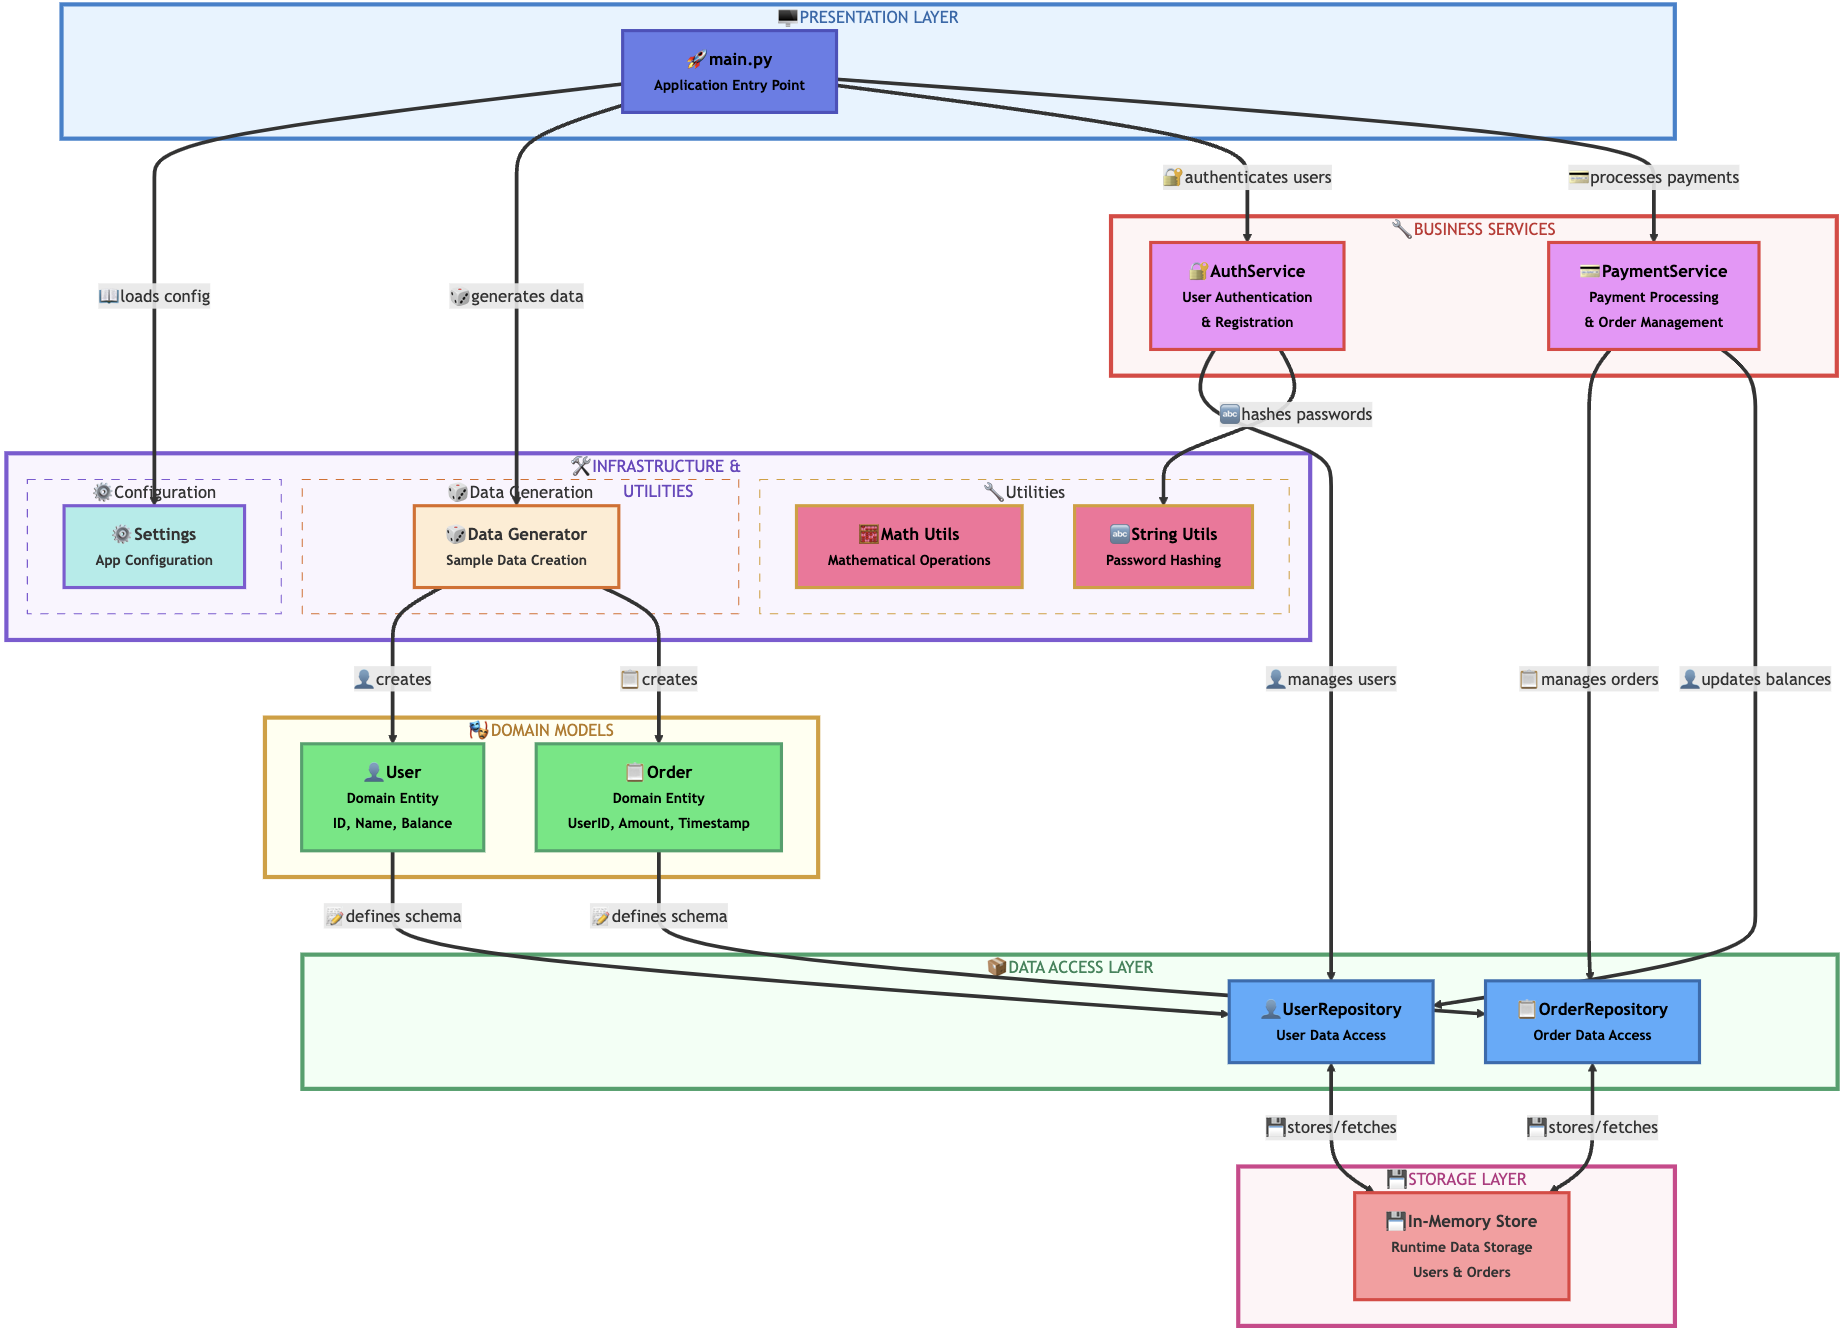
\includegraphics[width=1.09\linewidth]{imgs/eps/repository_visualization.eps}
    \caption{Project Repository Visualization}
    \label{fig:repository_visualization}
\end{figure}

Through these measures, we constructed a dataset that enables systematic evaluation of the impact of natural language and compression of natural language on test generation.

\subsection{Evaluation Metrics}

In this experiment, we evaluated performance using the following three primary metrics: token count, API cost, and code coverage.

\begin{enumerate}
    \item Token Counts + API Costs
\vspace{0.2cm}
    \item Number of Requests
\vspace{0.2cm}
    \item Code Coverage
\end{enumerate}

During the experiment, we recorded the cumulative token count and API cost required for Cline to generate and iteratively refine test code until it executed without errors. These values were compared against the final achieved values for each configuration.

The total token count per input prompt is defined as:

\[
\text{Input Prompt}
  = \text{Source Code}
  + \text{Prompt}
  + \text{Docstrings (if present)}
  + \text{Error Report}
\]

\subsection{Experimental Procedure}
Figure \ref{fig:experiment_overview} shows the overall experimental procedure. As shown by the structure of the dataset, we evaluated three different test case generation methods using LLMs:

\begin{figure}[htbp]
    \centering
    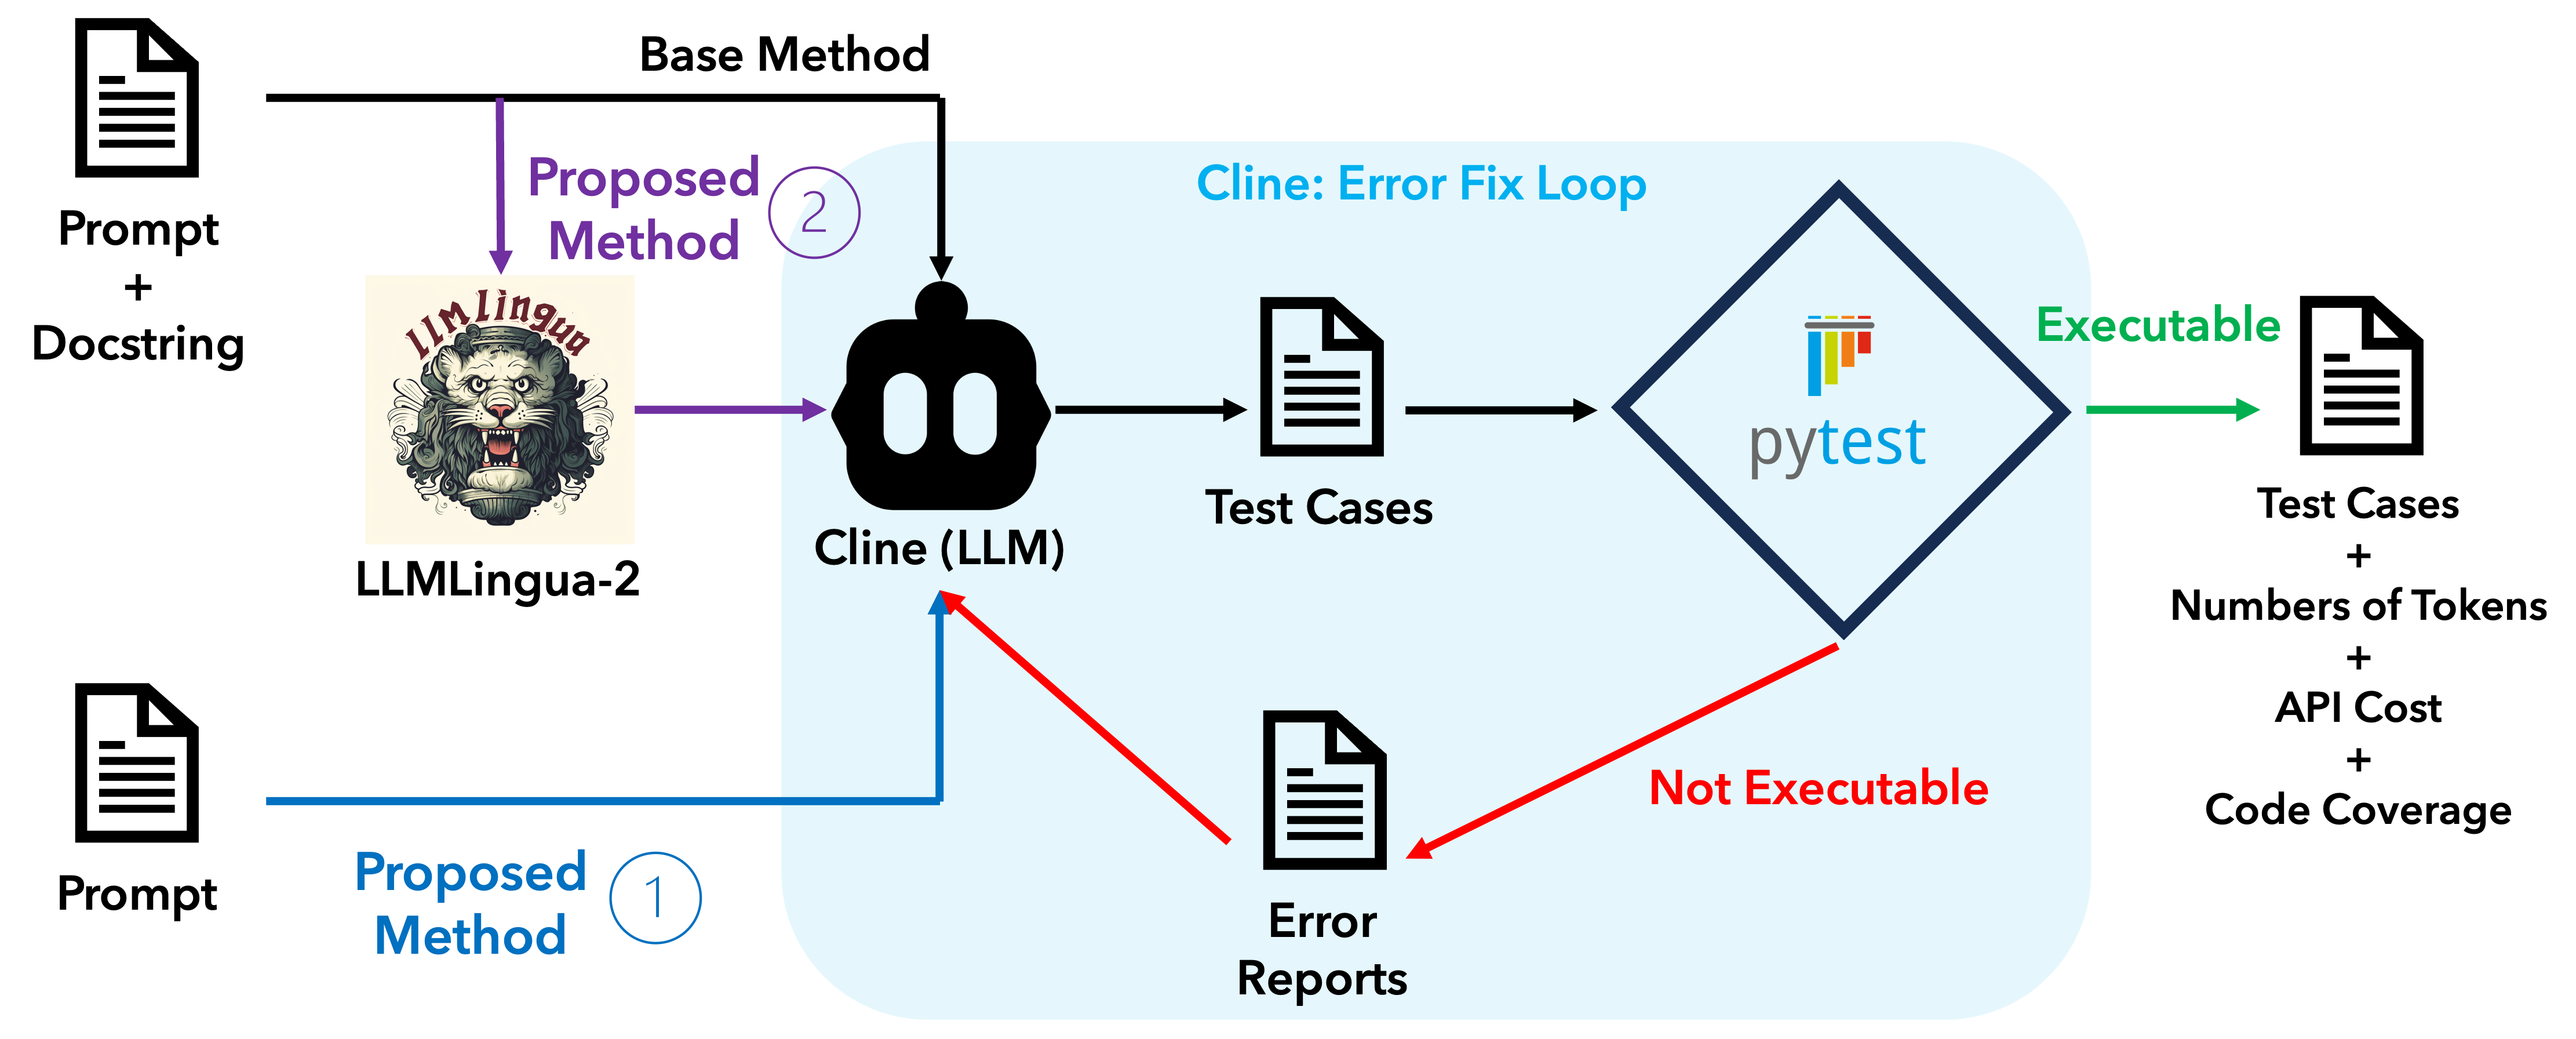
\includegraphics[width=1.0\linewidth]{imgs/png/overview_old.png}
    \caption{Experiment Overview}
    \label{fig:experiment_overview}
\end{figure}

\begin{itemize}[label={$\bullet$}]
    \item \textbf{Base Method}: \\Test cases are generated by providing LLMs with source code that includes both the prompt and docstrings.
\vspace{0.2cm}
    \item \textbf{Proposed Method 1}: \\Docstrings are removed from the code, and only the prompt is provided to LLMs.
\vspace{0.2cm}
    \item \textbf{Proposed Method 2}: \\The same prompt and docstrings used in the Base Method are compressed using LLMLingua-2 before being provided to LLMs.
\end{itemize}

As described earlier, an AI agent framework is used to iteratively generate and fix test cases until they execute correctly. The correctness of generated test cases is verified using a Pytest-based environment.


\section{Results}
    Tables \ref{table:results_base}–\ref{table:results_llmlingua} show the raw outcomes for the base method and the three proposed method. 

\begin{table}[htbp]
  \centering
  \caption{Token usage, API cost, and request count - Base Method}
  \begin{tabular}{
      l
      c@{\hspace{0.5em}}c@{\hspace{0.5em}}c@{\hspace{1em}}   % Claude   : Tokens ⟶ gap ⟶ Cost, Req.
      c@{\hspace{0.5em}}c@{\hspace{0.5em}}c@{\hspace{1em}}   % Gemini   : Tokens ⟶ gap ⟶ Cost, Req.
      c@{\hspace{0.5em}}c@{\hspace{0.5em}}c   % GPT-4.1 : Tokens ⟶ gap ⟶ Cost, Req.
    }
    \toprule
          & \multicolumn{3}{c}{Claude 3.7 Sonnet}
          & \multicolumn{3}{c}{Gemini 2.5 Pro Preview}
          & \multicolumn{3}{c}{GPT-4.1} \\
    \cmidrule(lr){2-4}\cmidrule(lr){5-7}\cmidrule(lr){8-10}
    Run & Tokens & Cost(USD) & Req. & Tokens & Cost(USD) & Req. & Tokens & Cost(USD) & Req. \\
    \midrule
    1 & 427\,000 & 0.418 & 16 & 353\,000 & 0.363 & 14 & 319\,000 & 0.230 & 13 \\
    2 & 559\,000 & 0.672 & 19 & 643\,000 & 0.457 & 22 & 454\,000 & 0.313 & 14 \\
    3 & 370\,000 & 0.381 & 14 & 498\,000 & 0.410 & 18 & 374\,000 & 0.236 & 15 \\
    4 & 436\,000 & 0.404 & 16 & 340\,000 & 0.285 & 14 & 433\,000 & 0.267 & 17 \\
    5 & 587\,000 & 0.635 & 19 & 491\,500 & 0.371 & 18 & 386\,000 & 0.246 & 15 \\
    \midrule
    Average\hspace{0.5em} & 475\,800 & 0.502 & 16.8 & 465\,100 & 0.3772 & 17.2 & 393\,200 & 0.258 & 14.8 \\
    \bottomrule
  \end{tabular}
  \label{table:results_base}
\end{table}



\begin{table}[htbp]
  \centering
  \caption{Token usage, API cost, and request count - Proposed Method 1}
  \begin{tabular}{
      l
      c@{\hspace{0.5em}}c@{\hspace{0.5em}}c@{\hspace{1em}}   % Claude   : Tokens ⟶ gap ⟶ Cost, Req.
      c@{\hspace{0.5em}}c@{\hspace{0.5em}}c@{\hspace{1em}}   % Gemini   : Tokens ⟶ gap ⟶ Cost, Req.
      c@{\hspace{0.5em}}c@{\hspace{0.5em}}c                 % GPT-4.1  : Tokens ⟶ gap ⟶ Cost, Req.
    }
    \toprule
          & \multicolumn{3}{c}{Claude 3.7 Sonnet}
          & \multicolumn{3}{c}{Gemini 2.5 Pro Preview}
          & \multicolumn{3}{c}{GPT-4.1} \\
    \cmidrule(lr){2-4}\cmidrule(lr){5-7}\cmidrule(lr){8-10}
    Run & Tokens & Cost(USD) & Req. & Tokens & Cost(USD) & Req. & Tokens & Cost(USD) & Req. \\
    \midrule
    1 & 751\,000 & 0.576  & 23 & 682\,000 & 0.780 & 24 & 301\,000 & 0.223 & 13 \\
    2 & 329\,000 & 0.348  & 14 & 296\,000 & 0.217 & 13 & 296\,000 & 0.217 & 13 \\
    3 & 546\,000 & 0.503  & 19 & 478\,000 & 0.360 & 19 & 363\,000 & 0.233 & 15 \\
    4 & 449\,000 & 0.595  & 18 & 485\,333 & 0.452 & 19 & 373\,000 & 0.231 & 16 \\
    5 & 743\,000 & 0.701  & 23 & 580\,000 & 0.570 & 22 & 300\,000 & 0.223 & 13 \\
    \midrule
    Average\hspace{0.5em} & 563\,600 & 0.5446 & 19.4 & 504\,267 & 0.476 & 19.2 & 326\,600 & 0.225 & 14.0 \\
    \bottomrule
  \end{tabular}
  \label{table:results_prompt_only}
\end{table}



\begin{table}[htbp]
  \centering
  \caption{Token usage, API cost, and request count - Proposed Method 2}
  \begin{tabular}{
      l
      c@{\hspace{0.5em}}c@{\hspace{0.5em}}c@{\hspace{1em}}
      c@{\hspace{0.5em}}c@{\hspace{0.5em}}c@{\hspace{1em}}
      c@{\hspace{0.5em}}c@{\hspace{0.5em}}c
    }
    \toprule
          & \multicolumn{3}{c}{Claude 3.7 Sonnet}
          & \multicolumn{3}{c}{Gemini 2.5 Pro Preview}
          & \multicolumn{3}{c}{GPT-4.1} \\
    \cmidrule(lr){2-4}\cmidrule(lr){5-7}\cmidrule(lr){8-10}
    Run & Tokens & Cost(USD) & Req. & Tokens & Cost(USD) & Req. & Tokens & Cost(USD) & Req. \\
    \midrule
    1 & 377\,000 & 0.361 & 15 & 350\,000 & 0.395 & 14 & 409\,000 & 0.285 & 16 \\
    2 & 371\,000 & 0.289 & 15 & 453\,000 & 0.401 & 17 & 312\,000 & 0.195 & 13 \\
    3 & 561\,000 & 0.494 & 19 & 401\,500 & 0.398 & 16 & 314\,000 & 0.196 & 13 \\
    4 & 430\,000 & 0.654 & 16 & 677\,000 & 0.621 & 23 & 671\,000 & 0.414 & 23 \\
    5 & 612\,000 & 0.540 & 20 & 565\,000 & 0.511 & 20 & 321\,000 & 0.204 & 13 \\
    \midrule
    Average\hspace{0.5em} & 470\,200 & 0.4676 & 17.0 & 489\,300 & 0.4652 & 17.9 & 405\,400 & 0.259 & 15.6 \\
    \bottomrule
  \end{tabular}
  \label{table:results_llmlingua}
\end{table}

% \begin{figure}[htbp]
    \centering
    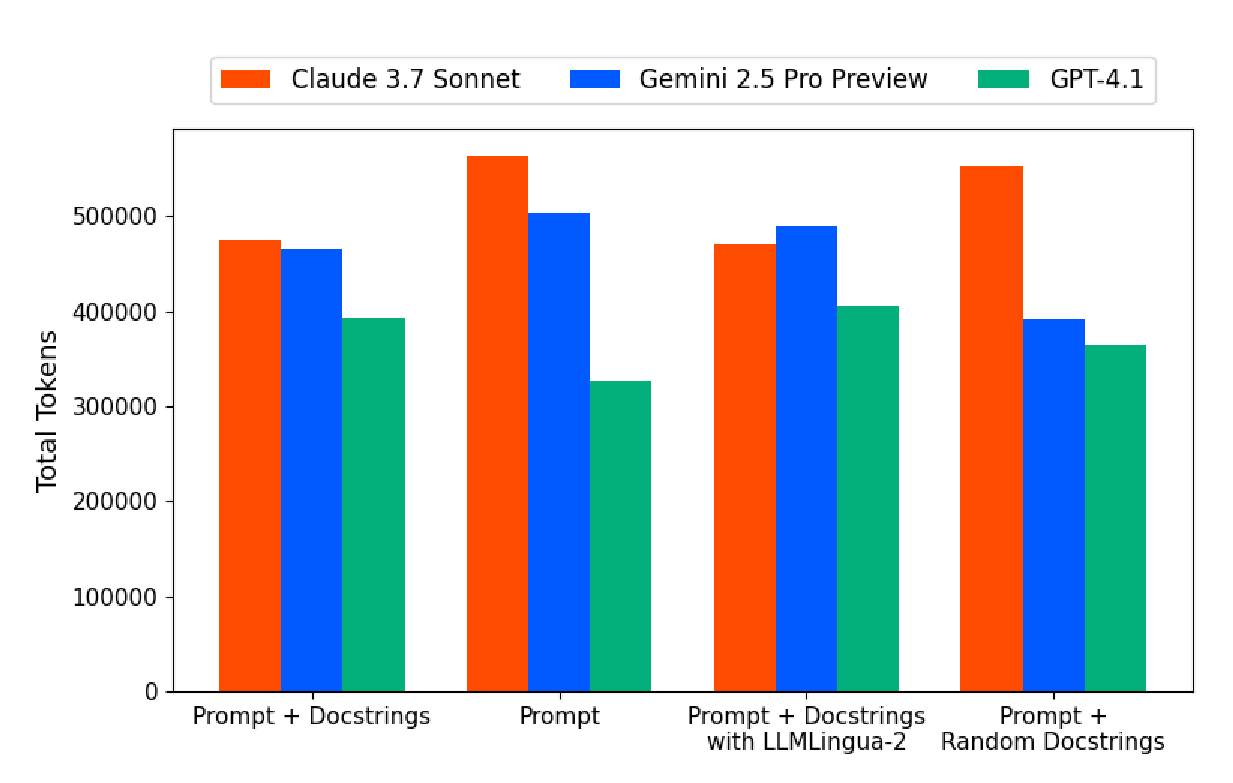
\includegraphics[width=0.9\linewidth]{imgs/eps/total_tokens_all.eps}
    \caption{Total Tokens}
    \label{fig:total_tokens}
\end{figure}

\begin{figure}[htbp]
    \centering
    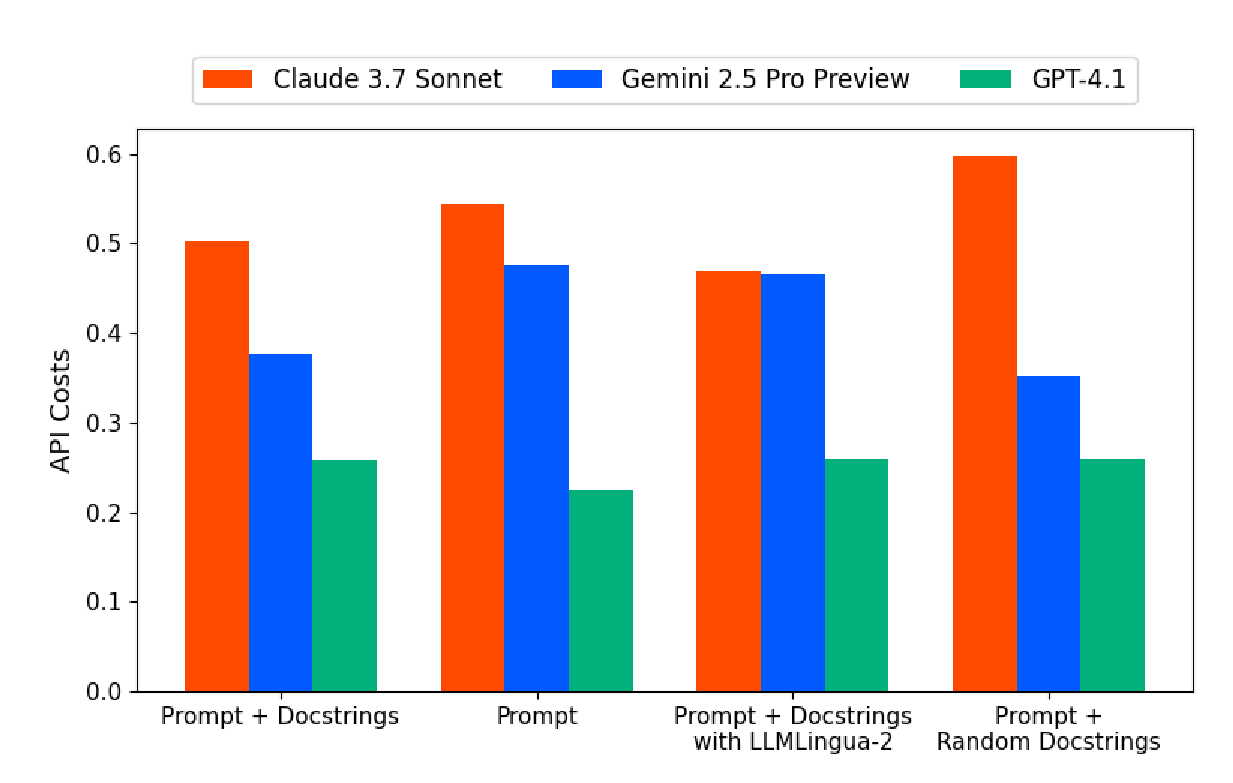
\includegraphics[width=0.9\linewidth]{imgs/eps/total_api_costs_all.eps}
    \caption{Total API Costs}
    \label{fig:total_api_costs}
\end{figure}

\begin{figure}[htbp]
    \centering
    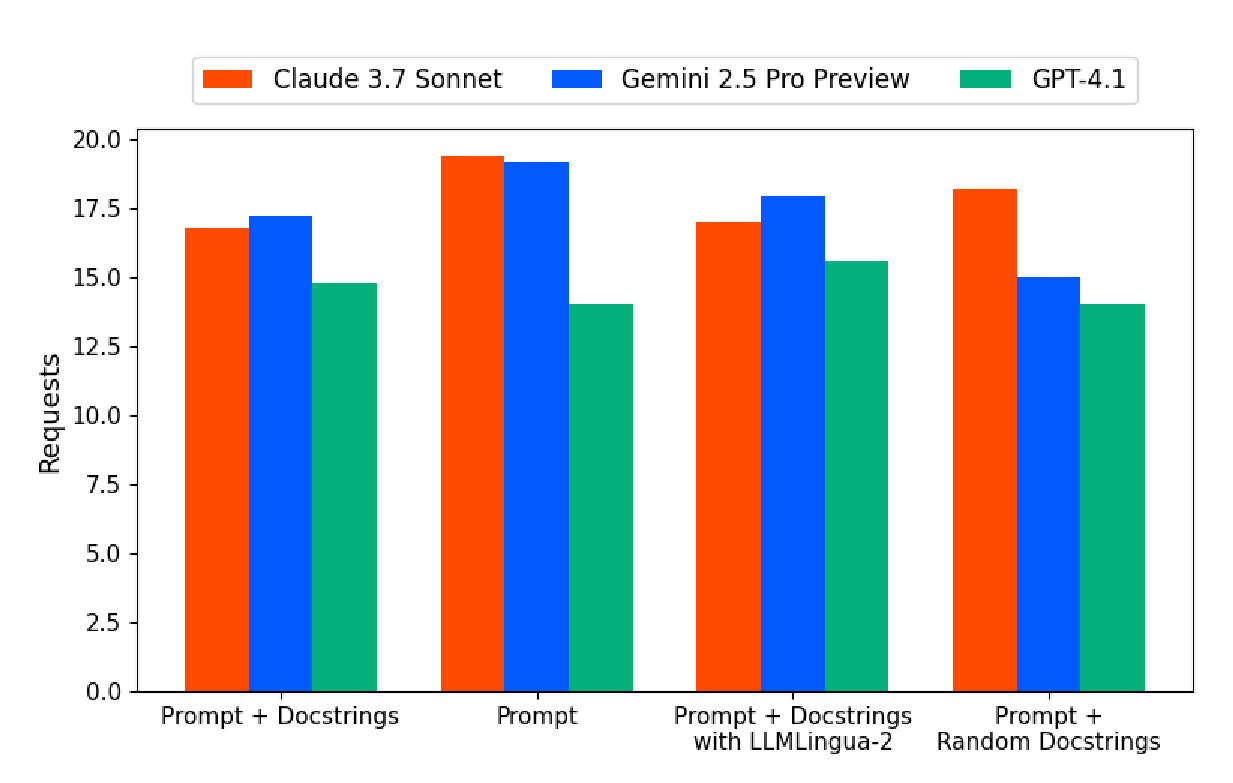
\includegraphics[width=0.9\linewidth]{imgs/eps/total_requests_all.eps}
    \caption{Total Requests}
    \label{fig:total_requests}
\end{figure}

\newpage

\subsection{Quantitative Comparison about Token Counts and API Costs, Number of Requests}

Table \ref{table:quantitative_comparison} shows the difference (\%) from the base method calculated based on the average values in Table \ref{table:results_base}-\ref{table:results_llmlingua}. PM means Proposed Method.

\begin{table}[h!]
    \centering
    \caption{Change Rates of LLM Performance Metrics (Relative to Base Method)}
    \begin{tabular}{lcccc}
        \toprule
        \textbf{LLMs} & \textbf{Metrics} \quad & \textbf{Base Method} & \textbf{PM1} & \textbf{PM2} \\
        \midrule
        \multirow{3}{*}{Claude 3.7 Sonnet} 
          & Tokens & 475{,}800 & \quad +18.4\% & \quad $-1.2$\% \\
          & Cost   & \$0.502 & \quad +8.6\% & \quad $-6.8$\% \\
          & Req.   & 16.8 & \quad +2.6 & \quad +0.2 \\
        \midrule
        \multirow{3}{*}{Gemini 2.5 Pro Preview} 
          & Tokens & 465{,}100 & \quad +8.4\% & \quad +5.2\% \\
          & Cost   & \$0.377 & \quad +26.2\% & \quad +23.3\% \\
          & Req.   & 17.2 & \quad +2.0 & \quad +0.7 \\
        \midrule
        \multirow{3}{*}{GPT-4.1} 
          & Tokens & 393{,}200 & \quad $-17.0$\% & \quad +3.1\% \\
          & Cost   & \$0.258 & \quad $-12.8$\% & \quad +0.4\% \\
          & Req.   & 14.8 & \quad $-0.8$ & \quad +0.8 \\
        \bottomrule
    \end{tabular}
    \label{table:quantitative_comparison}
\end{table}

Table \ref{table:impact_of_each_method} shows a summary of the performance impact of each proposed method from Table \ref{table:quantitative_comparison}. From Table \ref{table:impact_of_each_method}, we can see these things:

\begin{enumerate}
    \item \textbf{LLMs Dependency}
        \begin{itemize}[label={$\bullet$}]
            \item Claude 3.7 Sonnet and Gemini 2.5 Pro Preview rely heavily on Docstrings for code understanding. Removing them leads to more correction requests.
            \vspace{0.2cm}
            
            \item GPT-4.1 shows low dependence on Docstrings and may even treat them as a source of noise.
        \end{itemize}
\vspace{0.3cm}

    \item \textbf{LLMLingua-2 Compression as a “Safe Option”}
        \begin{itemize}[label={$\bullet$}]
            \item Produced the best results with Claude 3.7 Sonnet. With Gemini 2.5 Pro Preview and GPT-4.1, the changes were minor, and the quality (Req) was largely maintained.
            \vspace{0.2cm}
            
            \item Since there’s little risk of degradation, it is effective as a general-purpose prompt-engineering strategy for reducing API costs.
        \end{itemize}
\end{enumerate}

\begin{table}[ht]
  \centering
  \caption{Impact of Each Method on Token Usage, Cost, and Request Count (relative to base method)}
  \setlength{\tabcolsep}{8pt}         % horizontal padding per column
  \begin{tabularx}{\linewidth}{@{}l L L@{}}  % ← Y → L
    \toprule
    \textbf{LLMs} &
    \thead{PM 1\\Docstrings Removal} &
    \thead{PM 2\\LLMLingua-2 Compression} \\
    \midrule
    Claude &
    \hspace{1.8cm} \makecell[l]{
      $\times$ Tokens/ Cost/ Req \textbf{increase}\\[2pt]
      $\Rightarrow$ All metrics degraded
    } &
    \hspace{2.0cm} \makecell[l]{
      $\bigcirc$ Tokens $-1.2\%$\\
      $\bigcirc$ Cost $-6.8\%$\\
      $\triangle$ Req $\approx$ unchanged\\[2pt]
      $\Rightarrow$ \textbf{lowest cost}
    } \\
    \addlinespace[4pt]
    \midrule[0.2pt] 
    Gemini &
    \hspace{1.8cm} \makecell[l]{
      $\times$ All metrics degraded
    } &
    \hspace{2.0cm} \makecell[l]{
      $\times$ All metrics degraded
    } \\
    \addlinespace[4pt]
    \midrule[0.2pt] 
    GPT-4.1 &
    \hspace{1.8cm} \makecell[l]{
      $\bigcirc$ Tokens $-17\%$\\
      $\bigcirc$ Cost $-12.8\%$\\
      $\bigcirc$ Req slightly \textbf{reduce}\\[2pt]
      $\Rightarrow$ \textbf{overall best} for GPT-4.1
    } &
    \hspace{2.0cm} \makecell[l]{
      $\triangle$ Roughly identical to \\ \hspace{0.5cm}base method
    } \\
    \bottomrule
  \end{tabularx}
  \label{table:impact_of_each_method}
\end{table}


\subsection{Code Coverage}
Under all conditions, the generated test cases achieved 100\% code coverage, as measured using the Pytest library. This result indicates that, at least for the dataset used in this study, neither the presence nor absence of natural language information—nor its compression—affected the final coverage.

\subsection{Impact of Docstrings}
Figure \ref{fig:token_usage_comparison} shows token usage statistics—mean, variance, minimum, and maximum—comparing the Base Method and Proposed Method 1 (Docstrings removed). For Claude 3.7 Sonnet, removing Docstrings reduces the variability in token counts, indicating more stable outputs without in-code descriptions. In contrast, Gemini 2.5 Pro Preview and GPT-4.1 show little change in variability, whether Docstrings are present or not.

Figure \ref{fig:variablity_comparison} presents the coefficient of variation (CV), which normalizes spread relative to scale. CV can calculated by standard deviation ($\sigma$) divided by the mean ($\mu$) as shown below. Here, Claude’s coefficient jumps significantly when Docstrings are omitted, revealing its strong dependence on Docstrings for consistent code comprehension. Meanwhile, Gemini 2.5 Pro Preview and GPT-4.1 maintain low and nearly identical coefficients across both conditions, suggesting that Docstrings have minimal impact on their understanding and output stability.

\[
\mathrm{CV} = \frac{\sigma}{\mu}
\]

\begin{figure}[htbp]
    \centering
    \includegraphics[width=1.0\linewidth]{imgs/eps/token_usage_comparison.eps}
    \caption{Token Usage Comparison: Mean Values with Standard Deviation}
    \label{fig:token_usage_comparison}
\end{figure}



\begin{figure}[htbp]
    \centering
    \includegraphics[width=1.0\linewidth]{imgs/eps/variability_comparison.eps}
    \caption{Variability Comparison: Coefficient of Variation}
    \label{fig:variablity_comparison}
\end{figure}


\section{Conclusion}
    This study confirmed that careful prompt-engineering can meaningfully reduce cost of LLM-based automated test case generation while maintaining perfect effectiveness.

\begin{enumerate}
    \item \textbf{Docstrings removal} reduced tokens and cost for GPT-4.1 (–17\% tokens, –12.8\% cost) but raised both metrics for Claude 3.7 Sonnet and Gemini 2.5 Pro Preview, revealing model-specific dependence on in-code documentation.
    \vspace{0.3cm}
    
    \item \textbf{LLMLingua-2 compression} of prompts and Docstrings delivered the most consistent savings—up to a 6.8\% cost drop for Claude 3.7 Sonnet—with negligible quality impact, making it a low-risk default optimisation.
    \vspace{0.3cm}
    
    \item \textbf{Docstrings inclusion} notably enhanced code comprehension and output quality for Claude 3.7 Sonnet, leading to lower total token usage, reduced API costs, and fewer correction requests when compared to prompts without Docstrings.
\end{enumerate}

% volatile: 不安定な

These findings demonstrate that prompt-size control, particularly via lightweight compression, can make large-scale automated test case generation economically sustainable. Practitioners should start with compression, assess each model’s sensitivity to documentation, and escalate to more aggressive reductions only when coverage and stability stay intact.


\section{Future Works}
    We are considering the following three directions as potential areas for future research.

\begin{itemize}[label={$\bullet$}]
    \item \textbf{Testing with Datasets Containing Faulty Code} \\Investigate whether LLM-generated test cases can detect defects in flawed source code, rather than merely producing outputs that pass incorrect logic.
    \vspace{0.3cm}
    
    \item \textbf{Code Compression with Meta Large Language Model Compiler (LLM Compiler)} \\Use LLM Compiler to condense source code into a compact intermediate representation, achieving prompt compression and reducing tokens and API costs during LLM-based test case generation \cite{cummins2024metalargelanguagemodel}.
    \vspace{0.3cm}

    \item \textbf{Using Incorrect Docstrings} \\Examine whether and to what extent Docstrings contribute to the LLM’s code comprehension, even when the documentation is inaccurate.
\end{itemize}


%
% ---- Bibliography ----
%
% BibTeX users should specify bibliography style 'splncs04'.
% References will then be sorted and formatted in the correct style.
%
% \bibliographystyle{splncs04}
% \bibliography{references}

\printbibliography

% \section{Appendix}
%     \input{chapters/09_appendix}

\end{document}
